\documentclass[runningheads,a4paper]{llncs}

\usepackage{amssymb}
\setcounter{tocdepth}{3}
\usepackage{graphicx}

\usepackage{url}
\newcommand{\keywords}[1]{\par\addvspace\baselineskip
\noindent\keywordname\enspace\ignorespaces#1}

% Additional packages
\usepackage[utf8]{inputenc}
\usepackage[round]{natbib}
\usepackage{subfig}
\usepackage{tikz}
\usepackage[pdftex,pdfpagelabels,bookmarks,hyperindex,hyperfigures]{hyperref}
\hypersetup{%
   plainpages=false, 
   pdfpagelayout=SinglePage,
   bookmarksopen=false,
   bookmarksnumbered=true,
   breaklinks=true,
   linktocpage,
   colorlinks=true,
   linkcolor=blue,
   urlcolor=blue,
   citecolor=blue,
   anchorcolor=green
}      

% TiKZ styles
\tikzstyle{var} = [circle,
                   thick,
                   draw, fill=red!20,
                   font=\scriptsize,
                   text width=3.5em,
                   text centered,
                   node distance=1em,
                   inner sep=0pt]

\tikzstyle{factor} = [rectangle,
                      thick,
                      draw, fill=blue!20,
                      minimum height=2em,
                      minimum width=2em]

\tikzstyle{line} = [draw]

\begin{document}

\mainmatter  % start of an individual contribution

% first the title is needed
\title{Using Graphical Models for Novelty Detection on Semantic Room Classification}

% a short form should be given in case it is too long for the running head
% \titlerunning{Lecture Notes in Computer Science: Authors' Instructions}

% the name(s) of the author(s) follow(s) next
%
% NB: Chinese authors should write their first names(s) in front of
% their surnames. This ensures that the names appear correctly in
% the running heads and the author index.
%
\author{André Susano Pinto}
%
%\authorrunning{Lecture Notes in Computer Science: Authors' Instructions}
% (feature abused for this document to repeat the title also on left hand pages)

% the affiliations are given next; don't give your e-mail address
% unless you accept that it will be published
\institute{Faculdade de Engenharia da Universidade do Porto, Portugal\\
\url{andresusanopinto@gmail.com}\\
\url{http://url}}

\toctitle{Lecture Notes in Computer Science}
\tocauthor{Authors' Instructions}
\maketitle


\begin{abstract}
This papers presents an approach on implementing novelty detection for indoor room classification
using semantic data.
\emph{Graphical models} are used to model probabilistic knowledge and a novelty threshold is
defined in terms of conditional and unconditional probabilities.
The novelty threshold is then optimized using an unconditional probability density
model trained from unlabelled data.


\keywords{novelty detection, semantic data, probabilistic graphical models,
room classification, indoor environments, robotics, multi-modal classification.}
\end{abstract}


%%%%%%%%%%%%%%%%%%%%%%%%%%%%%%%%%%%%%%%%%%%%%%%%%%%%%%%%%%%%%%%%%%%%%%
\section{Introduction}
There has been several efforts in the area of Artificial Intelligence and Robotics in creating
robots that are able to interact with humans and their environments.
One of the existing problems is a reliable high-level localization method that can be deployed
into new and unknown environments.
This article focus on the mapping, using \emph{semantic data}, of indoor environments such as
houses and offices to room categories such as kitchen, corridor, office.
And how to perform novelty detection on them: \emph{detect a new room category that was not
present in the labelled data}.

Dora\cite{dora} (CogX: Dora) was used as a base system where to implement the presented novelty
detection system.
As Dora moves through the environment its \emph{conceptual layer} builds a structural and
probabilistic representation of the space instantiated as a \emph{graphical model}.
That model connects the sensed properties together with the variables used to model the world.
And allows to perform queries on the probabilities of aspects of the environment.
For example: where is most likely to find a cereal box\cite{exploiting}.

The ability to recognize novel categories on the modelled variables would allow to increase
reliability and allow the creation of self-extending behaviours.


%%%%%%%%%%%%%%%%%%%%%%%%%%%%%%%%%%%%%%%%%%%%%%%%%%%%%%%%%%%%%%%%%%%%%%
\section{Related Work}
\cite{quattoni2009recognizing} showed that most scene recognition models work poorly in indoor
scenes when compared to outdoor scenes results.
Since the properties that characterize rooms changes conforming its category. Namely corridors are
well described by global properties and bookstores are well described by the presence of specific objects (books).
Their work shows a multi-modal approach is expected to yield better performance by mixing several sources of information.

\cite{galindo2005multi} defines a bidirectional relation between object and room category, where object defines a room category and a room category provides information on where objects may be found.

Probabilistic representations are used in several localised functions in robots operating in the real-world~\cite{gross2009toomas,maierprobabilistic}. And some employ, up to some extent, a probabilistic representation across some subsystems~\cite{kraft2008exploration}.
\cite{vasudevan2008bayesian} performed room categorization through Bayesian reasoning about the presence of objects but did not included observations models (perception is considered deterministic).
And \cite{boutell2006factor} have studied outdoor scene classification using \emph{factor graphs} and modelling spatial relations between objects in the scene to extract better knowledge from semantic (high-level) features.

Its expected that using a unified probabilistic model from the whole system, such as \cite{pronobis2011exploiting}, more information can be reused to correctly predict a given random variable.

Although this paper deals with novelty detection on the robotics area, it does so using very
standard concepts and techniques such as semantic data and graphical models.
Those are often found on areas related with information retrieval.
Interesting examples are works in automatic image annotation using an hidden concept layer between visual features and text information\cite{zhang2005probabilistic}.

%%%%%%%%%%%%%%%%%%%%%%%%%%%%%%%%%%%%%%%%%%%%%%%%%%%%%%%%%%%%%%%%%%%%%%
\section{Dora Architecture Overview}
Short paragraph describing dora. Short paragraph describing dora. Short paragraph describing dora. Short paragraph describing dora. Short paragraph describing dora.

From its architecture only the \emph{conceptual layer} is of interest to this article.
Its role is to aggregate the following semantic information coming from other layers:

\begin{description}
 \item[Doorway detection] is used to segment the low-level space into rooms and map connectivity between them.
 \item[Room size and shape] are classified by using 2D laser scans data and are associated as properties of a given room. The system utilizes pre-trained set of classifiers to label size as (large, medium, small) and shape as (rectangular or elongated).
 \item[Object detection] is performed using the visual input in order to detect . The system keeps track of the number of object and types seen per each room. Objects are once again detected by running a pre-trained set of detectors for: book, cereal box, computer, robot, stapler, toilet paper.
 \item[Room appearance] is categorized from the visual input by using CRFH and a pre-trained set of 7 different models.
\end{description}

With the extracted information and conceptual knowledge the conceptual layer creates a structured probabilistic representation
in order to model all known variables and their relations.
As so, in order to represent the knowledge the layer builds a \emph{chain graph}:
a probabilistic graphical model that merges both Bayesian Networks and Random Markov Fields.

The use of graphical models to describe distributions of variables has useful properties.
The edges between the variables can be seen as a kind of filter to the properties of the system.
Properties those that are expected to be captured by the conceptual knowledge.
At the same time they are a generative models and therefore allow to calculate the probability
on any given subset of variables on the graph allowing the system to work even when some
information is missing.


\begin{figure}[h]
\centering

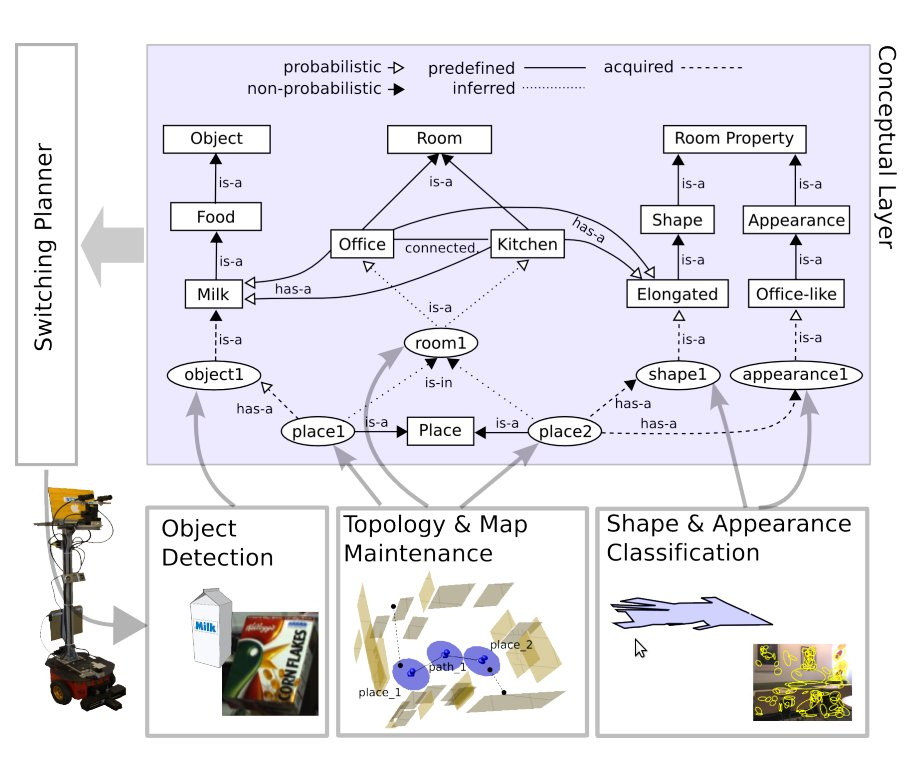
\includegraphics[width=0.50\textwidth]{figures/conceptual-layer.jpg}
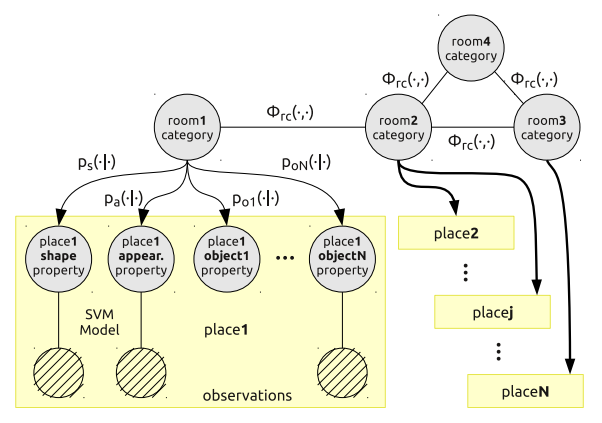
\includegraphics[width=0.49\textwidth]{figures/chain-graph.png}
\caption{The conceptual layer structures the sensed environment together with the conceptual knowledge
         in order to create a structured probabilistic representation of the world.}
\end{figure}

\subsection{Factor Graphs}
Although the conceptual layer works with \emph{chain graphs}, those can be converted into \emph{factor graphs}.
Those are used through this paper as they provide an easier manipulation in terms of factorization.

A \emph{factor graph} $G$ is a bipartite graph connecting a set of nodes $V_G$ representing
random variables and factors $\phi_G$.
Each factor represents a function dependent only on the variables to where its connected.
As so given factor graph $G$ can be seen as description of a distribution function over a set
of variables obtained by the product of all the factors. In order to represent a probability
a normalization factor $Z$ needs to be introduced:

\begin{equation}
P_G(X_V) = \frac{1}{Z}\prod_{}{\phi(...)},\qquad Z = \sum\prod{\phi(...)}
\end{equation}

Describing the distribution function in terms of graphs allows to use algorithms such as the
Sum-Product to efficiently calculate marginals on any given subset $x$ of variables by
exploiting conditional independency between variables.

\begin{equation}
P_G(x) = \frac{1}{Z}\sum_{V \\ x}{\prod{\phi(...)}}
\end{equation}

\begin{figure}[h]
\centering
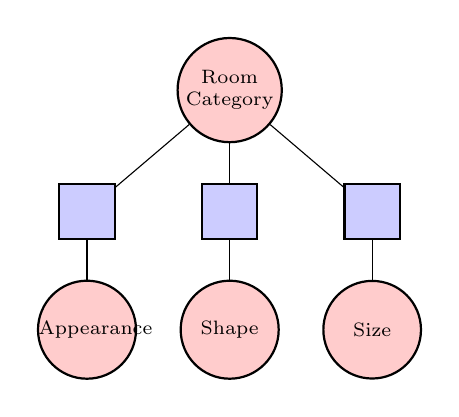
\begin{tikzpicture}[node distance = 2cm, auto]
    \matrix[row sep=0.5cm,column sep=0.5cm] {
      & \node [var] (room) {Room Category}; \\
      \node [factor] (fAppearance) {}; &
      \node [factor] (fShape) {}; &
      \node [factor] (fSize) {}; \\

      \node [var] (appearance) {Appearance}; &
      \node [var] (shape) {Shape}; &
      \node [var] (size) {Size}; \\
    };
  \path [line] (room) -- (fAppearance);
  \path [line] (room) -- (fShape);
  \path [line] (room) -- (fSize);

  \path [line] (fAppearance) -- (appearance);
  \path [line] (fShape) -- (shape);
  \path [line] (fSize) -- (size);
\end{tikzpicture}
\caption{Example of a factor graph used for Dora for representing the environment.}
\end{figure}

%%%%%%%%%%%%%%%%%%%%%%%%%%%%%%%%%%%%%%%%%%%%%%%%%%%%%%%%%%%%%%%%%%%%%%
\section{Novelty Detection}
% Introduce novelty detection
Novelty detection is an harder problem than that of classification due to its single-class nature.
Essentially a system is given training data and when given new data has to decide if it belongs
to the same concept it was trained with.

% Explain threshold approach to novelty detection
Due to the desire of robustness and generalization, a novelty detection system would always possess
some threshold that describes on how strict the system should be to new data.
This threshold is often seen as a distance measure to a normal input and several novelty detection
techniques are based on it.

When dealing with a statistic point of view, noisy data or unstable features, a decision on a
given input has an associated error rate. A novelty detection system is interested in defining an
order on all the possible inputs equivalent to the order imposed by the error rate: $P(novel|x)$.

Using bayes rule on the reversed order $P(\overline{novel}|x)$ and assuming a constant $P(\overline{novel})$
we obtain a ratio between a conditional and unconditional probabilities of the input $x$.
Such a ratio is a suitable function for implementing an optimal novelty detector system with
thresholding.

\begin{equation}
\label{eq:novelty-threshold}
          P(\overline{novel}|x)
  =       \frac{P(x|\overline{novel}) P(\overline{novel})}{P(x)}
  \propto \frac{P(x|\overline{novel})}{P(x)}
\end{equation}

% Explain approach of using conditional probability
\subsection{Conditional Probability: $P(x|\overline{novel})$}
\label{sec:uniform-unconditional}

One of the hardest problems is that on most cases a novelty detection system only has access to 
the known data.
Under that the best approach is to define a threshold based on $P(x|\overline{novel})/P(x)$
considering that $P(x)$ is constant through all the input space.

In the presented case the conditional probability is approximated by the graphical model $G$
produced by the conceptual layer.
The \autoref{fig:conditional-prob-graph} represents a possible graph $G$ built from the conceptual
layer to represent the conditional probability on the sensed variables $x$.
$P_G(x)$ is used as an approximation for $P(x|\overline{novel})$.

\begin{figure}[h]
\centering
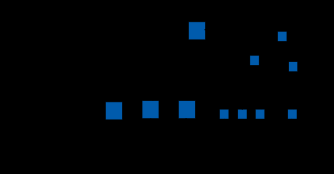
\includegraphics[width=0.70\textwidth]{figures/conditional-prob-graph.pdf}
\caption{\label{fig:conditional-prob-graph}The conceptual layer models the conditional
         probability distribution of the sensed variables by using hidden variables.
         Those are created from the conceptual knowledge and represent the structural
         and connectivity information the system is aware of.
         In this case only hidden variables $R_i$ were used to model the room categories
         where each property was sensed.}
\end{figure}


Its important to notice that in several cases assuming the unconditional probability $P(x)$
is constant leads to discarding the factor.
Nonetheless, here the distributions are dynamically changing as the system learns more on the environment.
So the normalizing argument $P(x)$ has to be evaluated for each new subset of $x$.

Assuming that the unconditional distributions generates all possible outcome with the same probability
we can model it with $\prod{1/\# x_i}$, where $\# x_i$ denotes the cardinality of the state space
of variable $x_i$.
In graphical model terms this is represented to a factor graph $U$ with the variables but
without any factors as illustrated on \autoref{fig:uniform-prob-graph}.

\begin{figure}
\centering
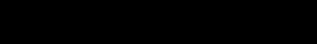
\includegraphics[width=0.70\textwidth]{figures/uniform-prob-graph.pdf}
\caption{\label{fig:uniform-prob-graph}Without any existing factors, this graph $U$ represents a
         uniform distribution over any set of its variables.}
\end{figure}

Having now a graphical model built to model the known data distribution and assuming that in the unconditional case all
possible outcomes are equally likely a novelty threshold would be given by: $P_G(x)/P_U(x)$.

Here $P_{U}(x)$ can be seen as a normalizing factor to lever all the $P_G(x)$ on any set of
variables $x$ into the same measure units (error rate), such that a static threshold can be implemented.
For example the conditional probability would yield very small values on large sets of variables
$x$ than in small sets due to the spreading over the dimensions of the input space.
As so a novelty measure is seen as a ratio on how much introducing the known concepts helps to
understand the observed result.


\subsection{Using Unlabelled Data}
Nonetheless its often the case that there is access to large amounts of unlabelled data.
Under that it becomes possible to obtain a better approach to the unconditional probability
distribution than the uniform one assumed in \autoref{sec:uniform-unconditional}.

For interesting and practical reasons it was assumed that the unconditional distribution
could be modelled with all the variables independent from each other.
Which translates as $P(x)=\prod{P_{x_i}(x_i)}$.
From the unlabelled data only the probability of each feature $x_i$ needs to be estimated.
\autoref{fig:semisupervised-threshold} illustrates a graph $I$ to model independent variables.

\begin{figure}[h]
\centering

\includegraphics[width=0.70\textwidth]{figures/independent-prob-graph.pdf}
\caption{\label{fig:semisupervised-threshold}Using unlabelled data, its possible to estimate
         the unconditional probability for each variable and this way try to compensate
         for a possible existent bias on some of the variables.}
\end{figure}

Once again the novelty threshold would be given by $P_G(x)/P_I(x)$.
This time the addition of the variables unconditional factors can be understood as an
attempt to compensate for an existing bias on the unconditional distribution.
Which is an important step to achieve a correct ordering of the input space for novelty
thresholding.


%%%%%%%%%%%%%%%%%%%%%%%%%%%%%%%%%%%%%%%%%%%%%%%%%%%%%%%%%%%%%%%%%%%%%%
\section{Results}
In order to verify the improvements obtained by using unlabelled data, a synthetic dataset
was generated.
The synthetic distribution assumes that an independent and variable size set of features
$x$ is generated by a given room category.
In whole there was 11 different room categories and 7 different measured properties types.

The known data was extracted by generating samples from 6 of the 11 classes.
Together with the generated known data, the room category that generated is given as label.
That known data is used to train factors to represent a conditional distribution.
Using unlabelled data, factors are trained to approximate an unconditional distribution
where all features are independent.
\autoref{fig:simple-experiment} shows the graph structure used for approximate the conditional and
unconditional distributions trained from the labelled and unlabelled data.

\begin{figure}[h]
\centering

\subfloat[Graph structure used to model conditional probability graph.
          The graph factors are trained using the labelled data.]{... conditional probability}
\qquad
\subfloat[Graph structure used to model unconditional probability graph.
          The graph factors are trained using the unlabelled data.]{... unconditional probability}

\caption{\label{fig:simple-experiment}The graph structures $G$ and $I$ used to model the
         conditional and unconditional probability.
         Note that graph $G$ correctly models the structure of the synthetic distribution, though
         during training it has not seen all possible room categories represented by variable $R_1$.}

\end{figure}

\begin{figure}[h!]
\centering
\includegraphics[width=0.60\textwidth]{results/synthetic-all.pdf}

\caption{\label{fig:synthetic-roc}ROC curve comparing novelty detection performance between an optimal detector,
         $P_G(x)/P_U(x)$ a graph ratio considering an uniform unconditional distribution and
         $P_G(x)/P_I(x)$ a graph ratio considering an independent unconditional distribution}
\end{figure}

Since the distribution is synthetic its possible to create an optimal novelty detector, as
its the error rate $P(novel|x)$ can be exactly measured.
That serves as a comparison on how optimal a detector can be using the same input space.
A ROC curve was plotted for the three methods on \autoref{fig:synthentic-roc}.
As possible to see the unconditional probability plays an important role in obtaining a correct
ordering of the input space.

The importance of a correct estimate of unconditional probability is expected to decrease as the
input space increases and allows the several existing classes to become easily distinguished.

For comparison ROC curves where plot for the developed threshold based on the number of input features.

\begin{figure}[h]
\centering

\subfloat[3 sensed variables]{\includegraphics[width=0.40\textwidth]{results/synthetic-3features.pdf}}
\qquad
\subfloat[5 sensed variables]{\includegraphics[width=0.40\textwidth]{results/synthetic-5features.pdf}}

\subfloat[10 sensed variables]{\includegraphics[width=0.40\textwidth]{results/synthetic-10features.pdf}}
\qquad
\subfloat[50 sensed variables]{\includegraphics[width=0.40\textwidth]{results/synthetic-50features.pdf}}

\caption{\label{fig:synthetic-roc-breakdown}ROC curves plotted showing performance of the
         presented novelty detection method on graphs generated for different amount of
         sensed variables.
         As possible to see as the system gains more semantic information it becomes easier
         to detect novelty and the effect of picking an approximation for the unconditional
         probability decreases.}
\end{figure}




%%%%%%%%%%%%%%%%%%%%%%%%%%%%%%%%%%%%%%%%%%%%%%%%%%%%%%%%%%%%%%%%%%%%%%
\section{Conclusions and Future Work}

On this paper it was presented how to define a stable novelty threshold function on top of
\emph{probabilistic graphical models} instantiated dynamically from sensed semantic data and
conceptual knowledge.
The presented technique is based on the ratio between a conditional and unconditional probability.

It was shown that unlabelled data can be used to approximate unconditional probability and
improve a novelty threshold.
And that a correct estimation of unconditional probability plays an important role specially on
small input spaces.

Future will work will focus on how to explain why a class is novel and what makes it different
other classes.
That will lead to generation of useful information that can be used on communication with the user
and perform active learning of new room categories.


%%%%%%%%%%%%%%%%%%%%%%%%%%%%%%%%%%%%%%%%%%%%%%%%%%%%%%%%%%%%%%%%%%%%%%
\bibliographystyle{plainnat}
\bibliography{refs}

\end{document}
